\newpage
\section{(R) Separation from Air Traffic}\label{sec:WellClear}

\paragraph{Remaining "Well Clear":} The separation from \emph{air traffic} is an activity when \emph{our airplane} tries to stay away from other traffic in safe manner.  

Before the definition of what is safe, there is a need for some margin definitions around the aircraft. The margins are enclosing a space in form of barrel, where \emph{airplane position} is center, the horizontal plane is base for circular boundary, the vertical axis is base for \emph{distance boundary} (fig. \ref{fig:WellClearTreshold}).

\begin{figure}[H]
    \centering
    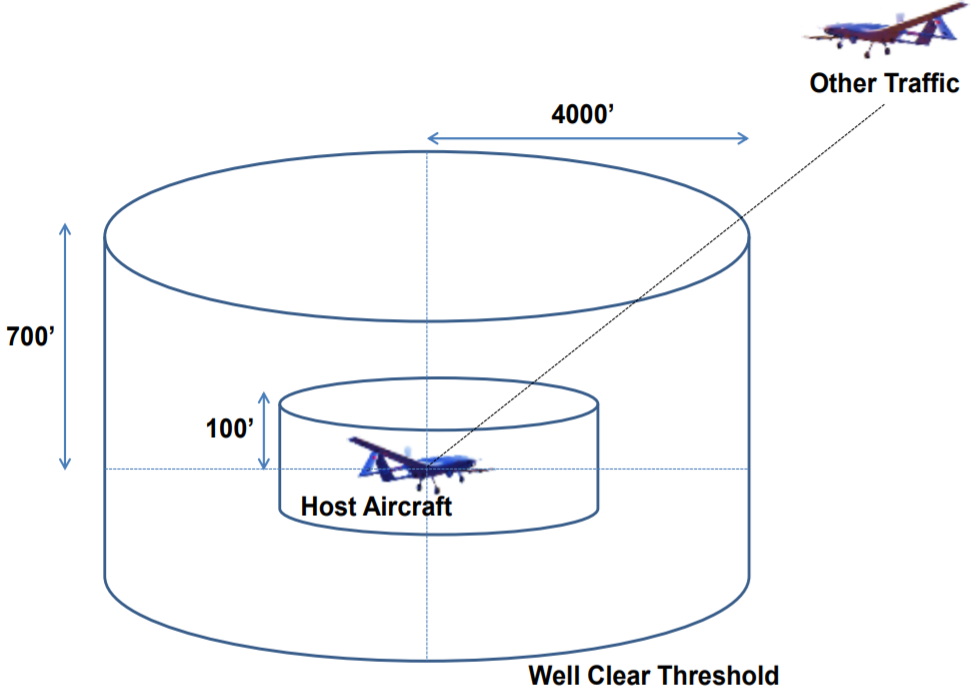
\includegraphics[width=0.6\textwidth]{\FIGDIR/02_05_WellClearTreshold}
    \caption{Well Clear Threshold \cite{valavanis2015uav,united1983pilots}.}
    \label{fig:WellClearTreshold}
\end{figure}

\noindent The boundaries and margins classification is taken from \cite{united1983pilots,valavanis2015uav} and goes like follow:

\begin{enumerate}
    \item \emph{"Alert"} - the distance to at least one surrounding aircraft is within \emph{alert margin}, the pilot is alerted about the possible threat, no action is required from pilot side.
    
    \item \emph{"Well Clear"} - the intruder enters into \emph{well clear range}, the intruder is threatening the \emph{airplane} directly, the pilot is noticed about security incident.
    
    \item \emph{"Near Miss"} - the intruder gets very close to \emph{airplane}, the body hit or \emph{turbulence impact} is very probable. 
    
    \item \emph{"Body Hit"} - the intruder stuck the \emph{airplane body}.
\end{enumerate}

\noindent These incidents are increasing their severity, the goal of separation is to keep every airspace attendant \emph{well clear}, outside well clear threshold (fig. \ref{fig:WellClearTreshold}). 
\paragraph{Air Traffic Control:} The air traffic control have passive role in separation, it manages the airspace and gives \emph{clearance} for air space users actions. There is active support for VFR (sec. \ref{sec:VisualFlightRules}) and IFR (sec. \ref{sec:InstrumentalFlightRules}). The role of \emph{Air Traffic Control} is discussed in (sec. \ref{sec:AirTrafficControl})

\paragraph{ACAS-X/TCAS:} There is support systems fo prevent \emph{Airborne Collision}, which are supporting the \emph{active avoidance} for \emph{IFR} flights (sec. \ref{sec:InstrumentalFlightRules}). Their role is to provide the surveillance of \emph{airplane} surroundings and give advisories to pilot. More about next generation system family ACAS-X can be read in (sec. \ref{sec:ACASX}). The current generation \emph{Airborne Collision} System TCAS is discussed in (sec. \ref{sec:TCAS}).

